\documentclass[aspectratio=169,11pt]{beamer}
% Shared preamble for the CogLean decks.
% Build the slides alone, or with speaker notes (see the Makefile):
%   pdflatex deck.tex                                   -> slides
%   pdflatex -jobname=deck-notes "\def\withnotes{}\input{deck.tex}"  -> slides + notes
\usetheme{default}
\usecolortheme{seahorse}
\setbeamertemplate{navigation symbols}{}
\setbeamertemplate{footline}[frame number]
\setbeamerfont{note page}{size=\small}
\ifdefined\withnotes
  \setbeameroption{show notes}
\fi
\usepackage[T1]{fontenc}
\usepackage{lmodern}
\usepackage{booktabs}
\usepackage{amsmath,amssymb}
\usepackage{tikz}
\usetikzlibrary{positioning,arrows.meta,shapes.misc}
\tikzset{
  box/.style={draw, rounded corners, align=center, minimum height=8mm, inner sep=4pt, fill=blue!6},
  arr/.style={-{Stealth[length=2mm]}, thick}
}
\newcommand{\code}[1]{\texttt{#1}}
\newcommand{\has}{\textbf{has}}
\newcommand{\lacks}{\textcolor{red!70!black}{lacks}}
\newcommand{\never}{\textcolor{red!70!black}{\textbf{never}}}
\newcommand{\canhold}{can hold}

% Lean source in slides: fvextra Verbatim, with the Unicode Lean uses mapped
% to math symbols (pdflatex).
\usepackage{fvextra}
\fvset{fontsize=\scriptsize, frame=single, framesep=2mm, rulecolor=\color{gray!50},
  breaklines=true, breakanywhere=false}
\DeclareUnicodeCharacter{2192}{\ensuremath{\to}}
\DeclareUnicodeCharacter{2190}{\ensuremath{\leftarrow}}
\DeclareUnicodeCharacter{2194}{\ensuremath{\leftrightarrow}}
\DeclareUnicodeCharacter{2200}{\ensuremath{\forall}}
\DeclareUnicodeCharacter{2203}{\ensuremath{\exists}}
\DeclareUnicodeCharacter{27E8}{\ensuremath{\langle}}
\DeclareUnicodeCharacter{27E9}{\ensuremath{\rangle}}
\DeclareUnicodeCharacter{2260}{\ensuremath{\neq}}
\DeclareUnicodeCharacter{2227}{\ensuremath{\wedge}}
\DeclareUnicodeCharacter{2228}{\ensuremath{\vee}}
\DeclareUnicodeCharacter{00AC}{\ensuremath{\neg}}
\DeclareUnicodeCharacter{2264}{\ensuremath{\le}}
\DeclareUnicodeCharacter{2208}{\ensuremath{\in}}
\DeclareUnicodeCharacter{2209}{\ensuremath{\notin}}
\DeclareUnicodeCharacter{00D7}{\ensuremath{\times}}
\DeclareUnicodeCharacter{03B1}{\ensuremath{\alpha}}
\DeclareUnicodeCharacter{03B2}{\ensuremath{\beta}}
\DeclareUnicodeCharacter{03BC}{\ensuremath{\mu}}
\DeclareUnicodeCharacter{03B8}{\ensuremath{\theta}}
\DeclareUnicodeCharacter{2218}{\ensuremath{\circ}}
\DeclareUnicodeCharacter{25B8}{\ensuremath{\blacktriangleright}}
\DeclareUnicodeCharacter{00B7}{\ensuremath{\cdot}}
\DeclareUnicodeCharacter{2026}{\ldots}


\title{Inside the proofs}
\subtitle{Recognition, retrieval and confident errors, in Lean\\\small(partner to ``Recognition, retrieval and confident errors'')}
\author{Jeff Shrager}
\date{October 2026}

\begin{document}

\begin{frame}
  \titlepage
\end{frame}
\note{
\begin{itemize}
\item This deck walks through the actual Lean code behind the companion talk. Code is quoted from the repository, lightly trimmed; ``-- ...'' marks omissions.
\item The point is architecture: how one behavioral theorem, confident errors, is assembled from small, general pieces, and then inherited.
\end{itemize}
}

\begin{frame}{The proof, layer by layer}
  \centering
  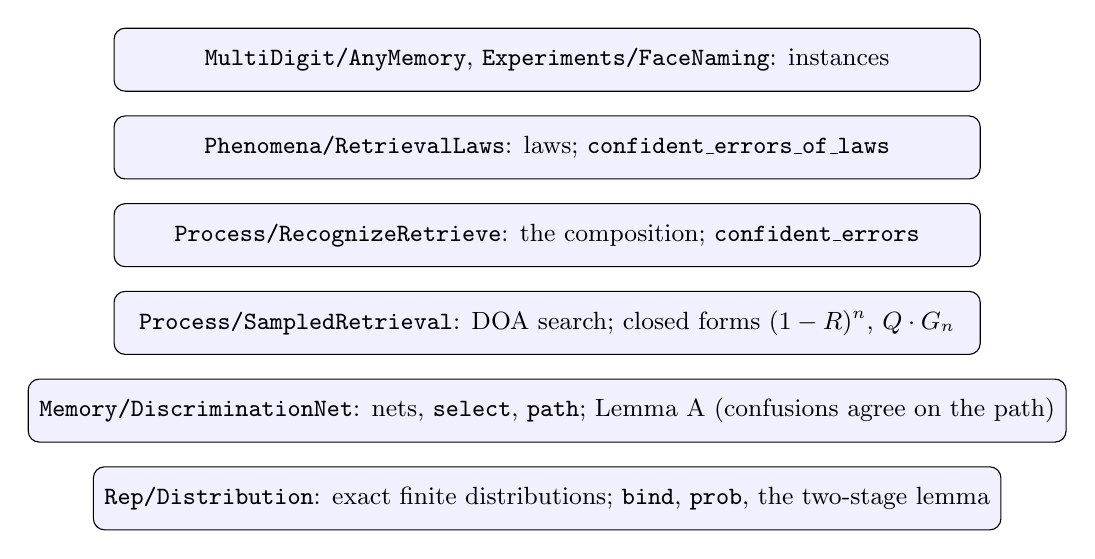
\begin{tikzpicture}[node distance=3mm, every node/.style={box, minimum width=11cm, font=\small}]
    \node (d) {\code{Rep/Distribution}: exact finite distributions; \code{bind}, \code{prob}, the two-stage lemma};
    \node[above=of d] (n) {\code{Memory/DiscriminationNet}: nets, \code{select}, \code{path}; Lemma A (confusions agree on the path)};
    \node[above=of n] (s) {\code{Process/SampledRetrieval}: DOA search; closed forms $(1-R)^n$, $Q\cdot G_n$};
    \node[above=of s] (c) {\code{Process/RecognizeRetrieve}: the composition; \code{confident\_errors}};
    \node[above=of c] (l) {\code{Phenomena/RetrievalLaws}: laws; \code{confident\_errors\_of\_laws}};
    \node[above=of l] (t) {\code{MultiDigit/AnyMemory}, \code{Experiments/FaceNaming}: instances};
  \end{tikzpicture}
\end{frame}
\note{
\begin{itemize}
\item Each layer imports only the ones below it. CogLib (the bottom five) imports no theory.
\item The top-level theorem's proof is a few lines because the work is factored into these layers, the way Mathlib factors algebra.
\end{itemize}
}

\begin{frame}[fragile]{Exact distributions}
\begin{Verbatim}
abbrev Dist (α : Type) := List (α × Rat)

/-- The distribution certain of `a`. -/
def pure (a : α) : Dist α := [(a, 1)]

/-- A two-stage process: draw `a` from `d`, then draw from `f a`. -/
def bind (d : Dist α) (f : α → Dist β) : Dist β :=
  match d with
  | [] => []
  | (a, p) :: d => ((f a).map fun (b, q) => (b, p * q)) ++ bind d f

/-- The probability of an event. -/
def prob : Dist α → (α → Bool) → Rat
  | [], _ => 0
  | (a, p) :: d, e => (if e a then p else 0) + prob d e
\end{Verbatim}
\end{frame}
\note{
\begin{itemize}
\item A distribution is a list of outcomes with exact rational probabilities. No floating point, no measure theory, no Mathlib.
\item Outcomes may repeat; an event's probability sums them. That keeps \code{bind} simple, at the cost of long lists when runs are computed.
\item Because everything is computable, the same definitions are run (\code{\#eval}) and proved about.
\end{itemize}
}

\begin{frame}[fragile]{The two-stage lemma}
\begin{Verbatim}
/-- A mixture: the probability of an event after a two-stage process is the
sum, over first-stage outcomes, of each one's probability times the event's
probability after it. -/
theorem prob_bind_sum (d : Dist α) (f : α → Dist β) (e : β → Bool) :
    prob (bind d f) e = (d.map fun ap => ap.2 * prob (f ap.1) e).sum := by
  induction d with
  | nil => simp [bind, prob]
  | cons x d ih => obtain ⟨a, p⟩ := x; rw [prob_bind_cons, ih]; simp
\end{Verbatim}
  \medskip
  Its specializations do most of the work above:
  \begin{itemize}\small
    \item \code{prob\_bind\_pure}: relabelling outcomes relabels the event;
    \item \code{prob\_bind\_split}: a second stage that is certain on one set of outcomes and constant on another.
  \end{itemize}
\end{frame}
\note{
\begin{itemize}
\item Induction on the list. The cons case uses \code{prob\_bind\_cons} (probability of the first outcome's branch, scaled, plus the rest), then the induction hypothesis.
\item Nearly every probabilistic proof in the talk reduces to this lemma or one of its specializations.
\end{itemize}
}

\begin{frame}[fragile]{Discrimination nets}
\begin{Verbatim}
inductive Net where
  | leaf : Option Item → Net
  | test : Feature → Net → Net → Net

/-- Selection: sort a code to a terminal and return its image. -/
def select : Net → Item → Option Item
  | leaf img, _ => img
  | test f n0 n1, x => if x.feat f then n1.select x else n0.select x

/-- The features examined while sorting `x`: the path it takes. -/
def path : Net → Item → List Feature
  | leaf _, _ => []
  | test f n0 n1, x => f :: (if x.feat f then n1.path x else n0.path x)
\end{Verbatim}
\end{frame}
\note{
\begin{itemize}
\item EPAM's net, directly: a terminal holds an image or nothing; a test branches on one binary feature.
\item Learning (\code{Net.learn}, not shown) replaces a confused terminal by a test on the first noticed difference.
\end{itemize}
}

\begin{frame}[fragile]{Lemma A: a confusion agrees on the path}
\begin{Verbatim}
theorem confusion_agrees_on_path (N : Net) (x y : Item) (hnd : N.images.Nodup)
    (hy : N.select y = some y) (hx : N.select x = some y) :
    ∀ f ∈ N.path x, x.feat f = y.feat f := by
  induction N with
  | leaf img => simp [path]
  | test f n0 n1 ih0 ih1 =>
    -- ...
    cases hxf : x.feat f <;> cases hyf : y.feat f <;> simp [hxf, hyf] at hx hy hg
    · -- both go to n0: the tested feature agrees, recurse
      rcases hg with rfl | hg
      · rw [hxf, hyf]
      · exact ih0 hnd0 hy hx g hg
    · -- x to n0, y to n1: y would be stored in both subtrees
      exact absurd rfl (hdisj y (select_mem_images n0 x y hx) y (select_mem_images n1 y y hy))
    -- ... (the two symmetric cases)
\end{Verbatim}
\end{frame}
\note{
\begin{itemize}
\item Structural induction on the net. At a test, case on the tested feature for $x$ and for $y$.
\item If they go the same way, the feature agrees and the induction hypothesis covers the rest of the path.
\item If they go different ways, $y$ would be stored on both sides, contradicting \code{Nodup} of the images. That hypothesis (each image stored once) is what EPAM's learning guarantees: \code{learnAll\_clean}.
\item This lemma is behind every near-miss prediction, and behind EPAM's \code{AgreesOn} law.
\end{itemize}
}

\begin{frame}[fragile]{DOA search, and a closed form}
\begin{Verbatim}
def search (as : List α) (s : α → Rat) (cc : Rat) : Nat → Nat → Dist (Retrieval α)
  | _, 0 => Dist.pure .exhausted
  | k, n + 1 => Dist.bind (sample as s) fun a =>
      if above s cc a then Dist.pure (.stated a (k + 1)) else search as s cc (k + 1) n

theorem prob_exhausted (as : List α) (s : α → Rat) (cc : Rat) (hT : total as s ≠ 0) :
    ∀ n k, prob (search as s cc k n) Retrieval.isExhausted = (1 - reach as s cc) ^ n := by
  intro n
  induction n with
  | zero => intro k; simp [search, prob_pure, Retrieval.isExhausted]
  | succ n ih =>
    intro k
    simp only [search]
    rw [prob_bind_split _ _ _ (fun _ => false) (fun a => !above s cc a) ((1 - reach as s cc) ^ n)]
    · rw [prob_false, prob_not_above as s cc hT, Rat.pow_succ]; grind
    · intro a
      by_cases ha : above s cc a
      · simp [ha, prob_pure, Retrieval.isExhausted]; grind
      · simp [ha, ih]; grind
\end{Verbatim}
\end{frame}
\note{
\begin{itemize}
\item Search is a recursive distribution: sample, state if above criterion, otherwise search again.
\item The closed form is proved by induction on the search length, splitting each step with \code{prob\_bind\_split}: above criterion ends the search (never exhausted), below it continues (exhausted with probability $(1-R)^n$ by induction).
\item The hypothesis \code{total $\neq$ 0} is real: with zero total strength, \code{sample} divides by zero. The blind simulation found that gap.
\end{itemize}
}

\begin{frame}[fragile]{The composition}
\begin{Verbatim}
def afterRecognition (str : Item → A → Rat) (as : List A) (cc : Rat) (n : Nat)
    (backup : P → Dist A) (x : P) : Option Item → Dist (Route × A)
  | none => Dist.bind (backup x) fun r => Dist.pure (.backup, r)
  | some y => Dist.bind (search as (str y) cc 0 n) fun
      | .stated a _ => Dist.pure (.whole, a)
      | .exhausted => Dist.bind (backup x) fun r => Dist.pure (.backup, r)

/-- Recognize, then retrieve, else back up. -/
def recognizeRetrieve (code : P → Item) (retrieve : Item → Dist (Option Item))
    (str : Item → A → Rat) (as : List A) (cc : Rat) (n : Nat) (backup : P → Dist A) (x : P) :
    Dist (Route × A) :=
  Dist.bind (retrieve (code x)) (RR.afterRecognition str as cc n backup x)
\end{Verbatim}
  \medskip
  Generic in the problem type \code{P}, the answer type \code{A}, and the memory (\code{retrieve}).
\end{frame}
\note{
\begin{itemize}
\item The composition is just \code{bind}: what memory calls up, then what follows.
\item Neither arithmetic nor EPAM appears here. Memory is any function from a probe to a distribution over stored codes.
\end{itemize}
}

\begin{frame}[fragile]{Confident errors: the proof is a composition}
\begin{Verbatim}
theorem confident_errors (correct : P → A) (x q : P) (hT : ∀ y, total as (str y) ≠ 0)
    (hbx : mass (backup x) = 1) (hbq : mass (backup q) = 1)
    (hq : retrieve (code q) = pure (some (code q)))
    (hx : retrieve (code x) = pure (some (code q)))
    (hs : Sharp str cc (code q) (correct q)) (hne : correct x ≠ correct q) :
    prob (recognizeRetrieve code retrieve str as cc n backup q) (wholeWrong correct q) = 0 ∧
      prob (recognizeRetrieve code retrieve str as cc n backup x) (wholeWrong correct x) =
        prob (recognizeRetrieve code retrieve str as cc n backup x) isWhole ∧
      prob (recognizeRetrieve code retrieve str as cc n backup x) isBackup =
        prob (recognizeRetrieve code retrieve str as cc n backup q) isBackup := by
  refine ⟨confusion_gives_neighbours_answer code retrieve str as cc n backup correct q q (hT _) hq hs,
    wrong_eq_whole_of_sharp code retrieve str as cc n backup correct x _ _ (hT _) hx hs hne, ?_⟩
  rw [backup_prob_certain code retrieve str as cc n backup x _ hx hbx hT,
    backup_prob_certain code retrieve str as cc n backup q _ hq hbq hT]
\end{Verbatim}
\end{frame}
\note{
\begin{itemize}
\item Three conjuncts, three earlier lemmas. The first is the neighbour's-answer lemma applied to $q$ itself; the second says that on sharp associations, every stated answer to $x$ is wrong; the third rewrites both backup probabilities to the same closed form $(1-R_q)^n$, after which the goal is an identity.
\item Note the hypotheses: retrieval is certain (\code{= pure (some \ldots)}). That is exactly what ACT-R never satisfies, and what the laws later supply.
\end{itemize}
}

\begin{frame}[fragile]{One supporting lemma}
\begin{Verbatim}
theorem confusion_gives_neighbours_answer (correct : P → A) (x q : P)
    (hT : total as (str (code q)) ≠ 0) (h : retrieve (code x) = pure (some (code q)))
    (hs : Sharp str cc (code q) (correct q)) :
    prob (recognizeRetrieve code retrieve str as cc n backup x)
      (wholeSuch fun a => a != correct q) = 0 := by
  rw [whole_depends_only_on_route code retrieve str as cc n backup x _ _ h,
    prob_stated _ _ _ _ hT]
  have : reachSuch as (str (code q)) cc (fun a => a != correct q) = 0 := by
    simp only [reachSuch]
    rw [prob_congr _ _ (fun _ => false), prob_false]
    intro a
    by_cases ha : above (str (code q)) cc a
    · simp [hs a ha]
    · simp [ha]
  rw [this]; grind
\end{Verbatim}
\end{frame}
\note{
\begin{itemize}
\item Step 1: whole-problem retrieval on $x$ is retrieval on $q$'s associations (\code{whole\_depends\_only\_on\_route}, itself from \code{recognizeRetrieve\_certain} and \code{bind\_pure\_left}).
\item Step 2: DOA's closed form for stating an answer with a property (\code{prob\_stated}): reach-with-property times a geometric factor.
\item Step 3: the reach for ``an answer other than $q$'s'' is zero, because sharpness says only $q$'s answer clears the criterion. Pointwise reasoning, then \code{prob\_false}.
\end{itemize}
}

\begin{frame}[fragile]{Memory as an interface}
\begin{Verbatim}
structure Retriever (State Stim : Type) where
  study : State → Stim → State
  retrieve : State → Stim → Dist (Option Stim)

-- EPAM: what a net's probe calls up, for certain
def Net.retrieve (N : Net) : Item → Dist (Option Item) := fun y => Dist.pure (N.select y)
def netRetriever (order : NoticingOrder) : Retriever Net Item := (netLearner order).toRetriever

-- ACT-R (decay 1, temperature 1): sample in proportion to weight, failure included
def retrieve (P : ActParams) (s : ActState) (x : Item) : Dist (Option Item) :=
  Dist.sample (outcomes s) (weight P s x)

/-- Retrieval is never certain. Failure is always among the outcomes. -/
theorem retrieve_not_certain (P : ActParams) (s : ActState) (x y : Item) :
    retrieve P s x ≠ Dist.pure (some y) := by
  intro h
  simp [retrieve, Dist.sample, outcomes, Dist.pure] at h
\end{Verbatim}
\end{frame}
\note{
\begin{itemize}
\item ACT-R's weight for a chunk is $\sum_k 1/(t - t_k)$ times $\mu^{\text{mismatches}}$, with a failure weight $\theta$: Boltzmann retrieval with decay 1 and temperature 1, exactly rational.
\item \code{retrieve\_not\_certain} is a one-line \code{simp}: the outcome list starts with \code{none}, so it can never equal \code{[(some y, 1)]}.
\end{itemize}
}

\begin{frame}[fragile]{The bridge to multi-digit addition}
\begin{Verbatim}
/-- The generic routes, in this model's names. -/
def relabel : Cog.Route × Nat → Route × Nat
  | (.whole, a) => (.whole, a)
  | (.backup, a) => (.columns, a)

theorem prob_trialWith (x : Problem) (e : Route × Nat → Bool) :
    prob (trialWith retrieve E str as cc n backup x) e =
      prob (recognizeRetrieve E.code retrieve str as cc n backup x) (fun o => e (relabel o)) := by
  unfold trialWith recognizeRetrieve
  rw [prob_bind_sum, prob_bind_sum]
  congr 1
  apply List.map_congr_left
  intro rp _
  rw [prob_after]

-- then each multi-digit theorem is two lines:
theorem confident_errors ... := by
  simp only [prob_trialWith, wholeWrong_relabel, isWhole_relabel, isColumns_relabel]
  exact RR.confident_errors E.code retrieve str as cc n backup Problem.sum x q ...
\end{Verbatim}
\end{frame}
\note{
\begin{itemize}
\item The multi-digit model keeps its own definitions and route names (so its exported numbers are byte-identical). One lemma carries every probability across, by the two-stage lemma on both sides.
\item Event identities (\code{isColumns} after relabelling is \code{isBackup}, and so on) are \code{funext} plus \code{cases}, closed by \code{rfl}.
\end{itemize}
}

\begin{frame}[fragile]{Laws}
\begin{Verbatim}
def Certainty (R : Retriever S Item) (s0 : S) (U : List Item) : Prop :=
  ∀ s, Reachable R s0 U s → ∀ y ∈ U, pRet R (R.study s y) y y = 1

def Stability (R : Retriever S Item) (s0 : S) (U : List Item) : Prop :=
  ∀ s, Reachable R s0 U s → ∀ y ∈ U, ∀ z ∈ U, z ≠ y → pRet R (R.study s z) y y = pRet R s y y

def Determinate (R : Retriever S Item) (s0 : S) (U : List Item) : Prop :=
  ∀ s, Reachable R s0 U s → ∀ x, ∃ r, R.retrieve s x = Dist.pure r

/-- Under determinacy, a positive chance of retrieving `y` is certainty. -/
theorem retrieve_of_pRet_pos (R : Retriever S Item) (s0 : S) (U : List Item)
    (hd : Determinate R s0 U) (s : S) (hs : Reachable R s0 U s) (x y : Item)
    (h : 0 < pRet R s x y) : R.retrieve s x = Dist.pure (some y)
\end{Verbatim}
  \medskip
  \small \code{pRet R s x y}: the chance that probe \code{x} retrieves \code{y}. \code{Reachable}: reached from \code{s0} by studying items of \code{U}.
\end{frame}
\note{
\begin{itemize}
\item Laws are \code{Prop}-valued definitions over the interface: no mechanism appears.
\item Each matrix cell is a theorem that a family's retriever has a law, or its negation.
\end{itemize}
}

\begin{frame}[fragile]{Studied items retrieve themselves}
\begin{Verbatim}
theorem studied_selfRetrieval (R : Retriever S Item) (s0 : S) (U : List Item)
    (hc : Certainty R s0 U) (hs : Stability R s0 U) (xs : List Item)
    (hU : ∀ x ∈ xs, x ∈ U) (hnd : xs.Nodup) (y : Item) (hy : y ∈ xs) :
    pRet R (R.studyAll s0 xs) y y = 1 := by
  obtain ⟨pre, post, hsplit⟩ := List.append_of_mem hy    -- xs = pre ++ y :: post
  -- ... y ∉ post, from Nodup
  rw [hsplit, show pre ++ y :: post = (pre ++ [y]) ++ post by simp,
    stable_after R s0 U hs y hyU post (pre ++ [y]) _ hpost,   -- studying post changes nothing
    studyAll_append]
  exact hc _ ⟨pre, hpre, rfl⟩ y hyU                            -- certainty, just after y
\end{Verbatim}
  \medskip
  \code{stable\_after} is an induction on \code{post}, applying stability once per item.
\end{frame}
\note{
\begin{itemize}
\item Split the study list at $y$. Certainty gives probability 1 just after $y$ is studied; stability, applied item by item to everything studied later (none of which is $y$, by \code{Nodup}), keeps it at 1.
\item This is also the whole content of the flat serial-position curve in the study-test experiment.
\end{itemize}
}

\begin{frame}[fragile]{Confident errors from laws}
\begin{Verbatim}
theorem confident_errors_of_laws (R : Retriever S Item) (s0 : S) (U : List Item)
    (hdet : Determinate R s0 U) (hcert : Certainty R s0 U) (hstab : Stability R s0 U)
    (xs : List Item) (hxs : ∀ y ∈ xs, y ∈ U) (hnd : xs.Nodup)
    (correct : P → A) (x q : P) (hq : code q ∈ xs)
    (hconf : 0 < pRet R (R.studyAll s0 xs) (code x) (code q))
    -- ... totals, backups, sharpness, correct x ≠ correct q
    := by
  have hr : Reachable R s0 U (R.studyAll s0 xs) := ⟨xs, hxs, rfl⟩
  have hq' := retrieve_of_pRet_one R s0 U hdet _ hr (code q) (code q)
    (studied_selfRetrieval R s0 U hcert hstab xs hxs hnd (code q) hq)
  have hx' := retrieve_of_pRet_pos R s0 U hdet _ hr (code x) (code q) hconf
  exact confident_errors code _ str as cc n backup correct x q hT hbx hbq hq' hx' hs hne
\end{Verbatim}
  \medskip
  Laws supply the two certain-retrieval hypotheses; the composition theorem does the rest.
\end{frame}
\note{
\begin{itemize}
\item This is where the matrix and the composition meet: \code{hq'} and \code{hx'} were per-state assumptions; now they are consequences of three laws and one observable fact (the stranger can be taken for $q$).
\item Only the discrimination family has all three laws.
\end{itemize}
}

\begin{frame}[fragile]{Using it: confident misnaming}
\begin{Verbatim}
theorem epam_confident_misnaming_of_laws (n : Nat) : ... :=
  RR.confident_errors_of_laws Person.face str names (1 / 2) n backup (netRetriever F3) (Net.leaf none)
    U3 (Discrimination.determinate F3 U3) (Discrimination.certainty F3 U3 noticeable_U3)
    (Discrimination.stability F3 U3) [ann.face, bob.face] (by decide) (by decide) Person.name carl bob
    (by decide) (by decide +kernel) total_ne (mass_backup carl) (mass_backup bob) sharp_bob
    (by decide)
\end{Verbatim}
  \medskip
  \begin{itemize}\small
    \item Three matrix cells for EPAM, cited by name.
    \item One computed fact, closed by \code{decide +kernel}: Carl's face can be taken for Bob's.
    \item No proof script: the theorem is a term, an application of the general result.
  \end{itemize}
\end{frame}
\note{
\begin{itemize}
\item The instance proof is a single application. The \code{by decide} side conditions are finite checks (list membership, no repeats, names differ).
\end{itemize}
}

\begin{frame}[fragile]{Computing inside the proof checker}
\begin{Verbatim}
theorem example_values :
    prob (trial bcd net str answers (1 / 2) 1 backup x) (wholeSuch (· == 200)) = 45 / 46 ∧
      prob (trial bcd net str answers (1 / 2) 1 backup x) (fun o => o.2 == 250) = 1 / 46 := by
  decide +kernel
\end{Verbatim}
  \medskip
  \begin{itemize}\small
    \item \code{decide +kernel}: the kernel evaluates the definitions and checks the equation. Plain \code{decide} gets stuck on \code{Rat}.
    \item The same definitions run under \code{\#eval}: the exported exact distributions that the blind simulation was checked against.
    \item Counterexample cells (``lacks'') are proved this way, on the eight 3-bit codes.
  \end{itemize}
\end{frame}
\note{
\begin{itemize}
\item Kernel evaluation is slow but trusted: no compiler or external solver is in the trusted base.
\item Because \code{Dist} doesn't merge duplicate outcomes, long computations grow; the exporter merges them, and needs a large stack.
\end{itemize}
}

\begin{frame}[fragile]{What is checked, and what is not}
\begin{Verbatim}
#print axioms Cog.RR.confident_errors_of_laws
'Cog.RR.confident_errors_of_laws' depends on axioms: [propext, Classical.choice, Quot.sound]
\end{Verbatim}
  \medskip
  \begin{itemize}
    \item No \code{sorry} anywhere; only Lean's three standard axioms.
    \item Core Lean only: no Mathlib, so everything computes.
    \item \textbf{Not checked}: that the definitions say what EPAM, DOA or ACT-R say. That is what the prose specification, the blind simulation, and (planned) comparison with PyACTUp are for.
  \end{itemize}
\end{frame}
\note{
\begin{itemize}
\item The three axioms are those every Lean development uses: propositional extensionality, choice, and quotient soundness.
\item Code: \code{CogLib/CogLib/Rep/Distribution.lean}, \code{Memory/DiscriminationNet.lean}, \code{Process/SampledRetrieval.lean}, \code{Process/RecognizeRetrieve.lean}, \code{Phenomena/RetrievalLaws.lean}; \code{MultiDigit/MultiDigit/AnyMemory.lean}; \code{Experiments/Experiments/FaceNaming.lean}.
\end{itemize}
}

\end{document}
